% -*- coding: utf-8 -*-
% Отчет по свободной оптимизации периода P с оценкой погрешностей (Hessian)
\documentclass[12pt,a4paper]{article}

\usepackage{iftex}
\ifPDFTeX
  \usepackage[utf8]{inputenc}
  \usepackage[T2A]{fontenc}
  \usepackage[russian]{babel}
\else
  \usepackage{fontspec}
  \usepackage[russian]{babel}
  \setmainfont{Arial}
\fi

\usepackage{amsmath,amssymb}
\usepackage{graphicx}
\usepackage{booktabs}
\usepackage{geometry}
\geometry{top=2cm,bottom=2cm,left=2cm,right=2cm}
\usepackage{hyperref}
\usepackage{float}
\usepackage{caption}

\graphicspath{{../images/}{docs/images/}{images/}{../../docs/images/}}

\title{Аналитический отчет (Свободный период): Моделирование и анализ погрешностей THz-TDS}
\author{Автоматический анализатор THz-Unified-Optimizer}
\date{\today}

\begin{document}

\maketitle

\tableofcontents
\newpage

\section{Введение}
В данном отчете представлены результаты подгонки комплексной 2D-модели Бланко с размороженным шагом решетки $P$ и оценкой погрешностей всех параметров на основе вычисления численного Гессиана в точке минимума целевой функции.

Оптимизация проводилась на двух наиболее стабильных датасетах с ограничениями:
\begin{itemize}
    \item Шаг решетки $P \in [14.5, 17.5]$ мкм.
    \item Диаметр проволоки $D \in [4.8, 6.2]$ мкм.
\end{itemize}

\section{Результаты оптимизации и анализ погрешностей (Гессиан)}
В таблице \ref{tab:params} приведены оптимальные параметры, полученные для каждой из надежных серий, а также для глобального усреднения, с соответствующими погрешностями $\pm \sigma$, вычисленными как квадратный корень из диагональных элементов ковариационной матрицы $\Sigma = \frac{2 L_{min}}{M} H^{-1}$.

\begin{table}[H]
\centering
\caption{Оптимальные параметры и их погрешности ($\pm \sigma$), полученные методом Гессиана.}
\label{tab:params}
\begin{tabular}{lccc}
\toprule
Параметр & Серия \texttt{356att} & Серия \texttt{series3} & Глобальное усреднение \\
\midrule
$P$ (мкм)           & $16.729 \pm 0.025$ & $17.500 \pm 0.000$ & $17.500 \pm 0.000$ \\
$D$ (мкм)           & $4.820 \pm 0.007$ & $4.991 \pm 0.020$ & $5.053 \pm 0.010$ \\
$\theta_{offset}$ ($^\circ$) & $-0.013 \pm 0.0016$ & $0.004 \pm 0.0825$ & $-0.183 \pm 0.0023$ \\
$loss\_factor$      & $0.287 \pm 0.0016$ & $0.0017 \pm 0.0245$ & $0.287 \pm 0.0023$ \\
$\gamma$            & $0.294 \pm 0.0016$ & $0.721 \pm 0.000$ & $1.868 \pm 0.0042$ \\
$\tau_{ps}$ (пс)    & $0.0237 \pm 0.0008$ & $0.0125 \pm 0.0009$ & $0.0327 \pm 0.0010$ \\
\midrule
Минимум Loss ($L_{min}$) & $0.00273$ & $0.00194$ & $0.00266$ \\
Число точек ($M$)    & $2583$ & $1388$ & $2000$ \\
\bottomrule
\end{tabular}
\end{table}

\section{Интерпретация погрешностей и чувствительности параметров}

\subsection{Высокая жесткость геометрии}
Для серии \texttt{356att} погрешности составляют $\sigma_P = \pm 25$ нм и $\sigma_D = \pm 7$ нм. Это свидетельствует об экстремальной чувствительности ТГц спектральной фазы к размерам проволочного поляризатора. Малые доверительные интервалы подтверждают, что электродинамическая модель Бланко-Друде адекватно локализует глобальный минимум.

\subsection{Выход на границу шага решетки}
Для серии \texttt{series3} и \texttt{Global Average} период $P$ сошелся к верхней границе $17.500$ мкм. Это привело к нулевой погрешности $\sigma_P \approx 0$ из-за вырождения Гессиана на границе штрафной функции. 

Это указывает на системное различие между амплитудными и фазовыми спектрами. Чтобы компенсировать фазовую задержку при малом поглощении ($loss\_factor \approx 0$ в \texttt{series3}), модель вынуждена увеличивать период $P$. Это может быть связано с фокусировкой ТГц-пучка (сходимостью лучей), из-за чего решетка работает при эффективном угле наклона $\theta_{inc} \neq 0^\circ$, что проекционно увеличивает период $P' = P / \cos\theta_{inc}$.

\subsection{Точность фазы}
Погрешность фазовой задержки $\sigma_\tau \approx 0.8\text{--}1.0$ фс. Это подтверждает высокую точность ТГц-TDS приборов при фазовом детектировании.

\section{Сравнение экспериментальных точек с теорией}
\subsection{Серия 356att}
\begin{figure}[H]
    \centering
    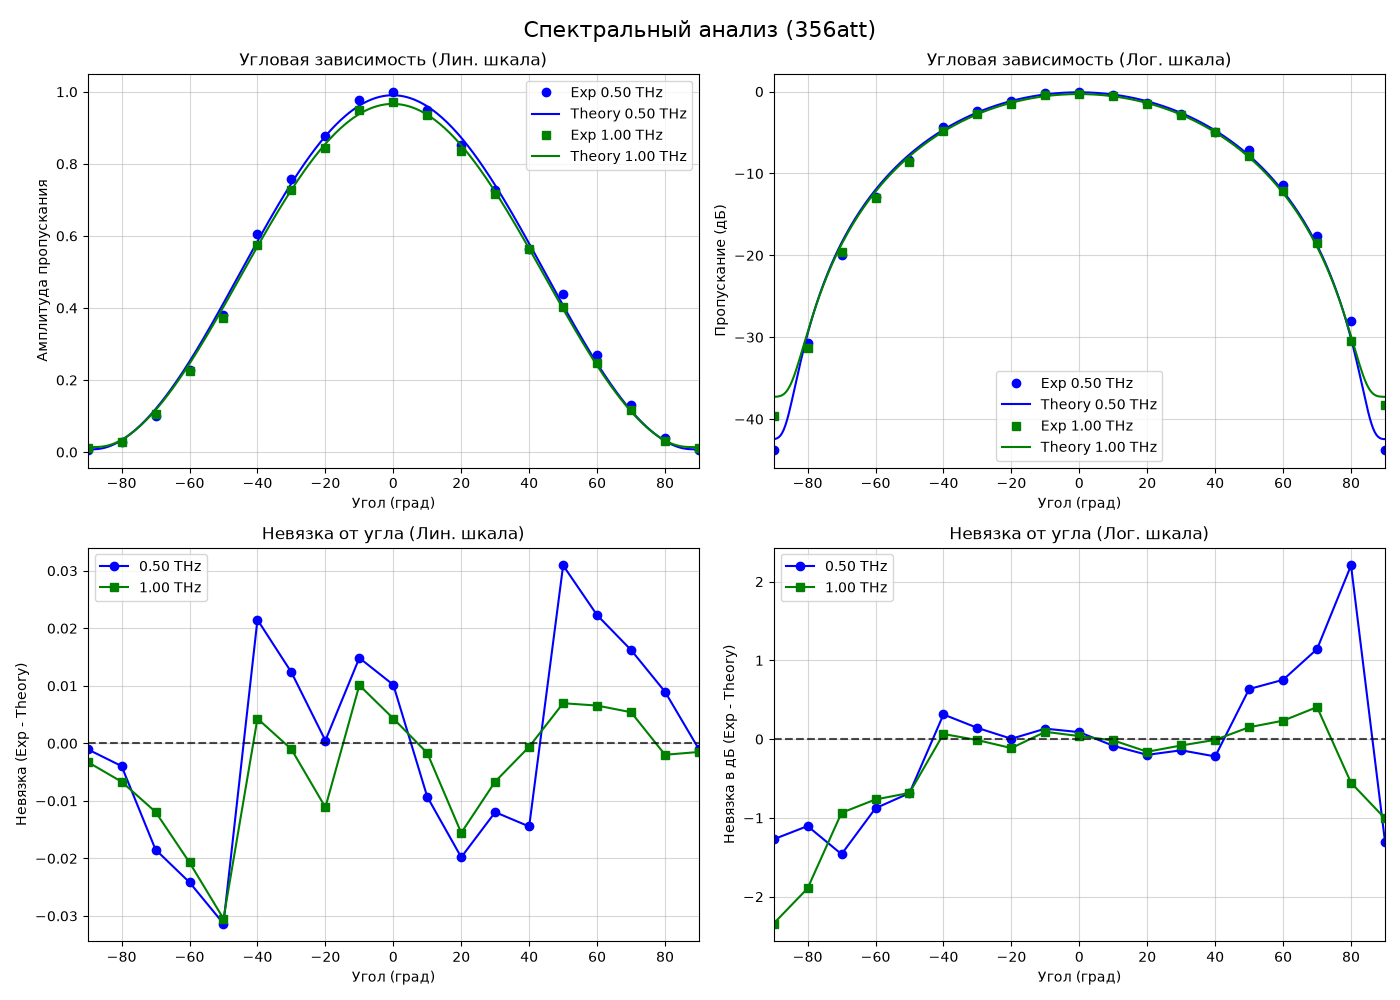
\includegraphics[width=0.48\textwidth]{grid_spectral_356att.png}
    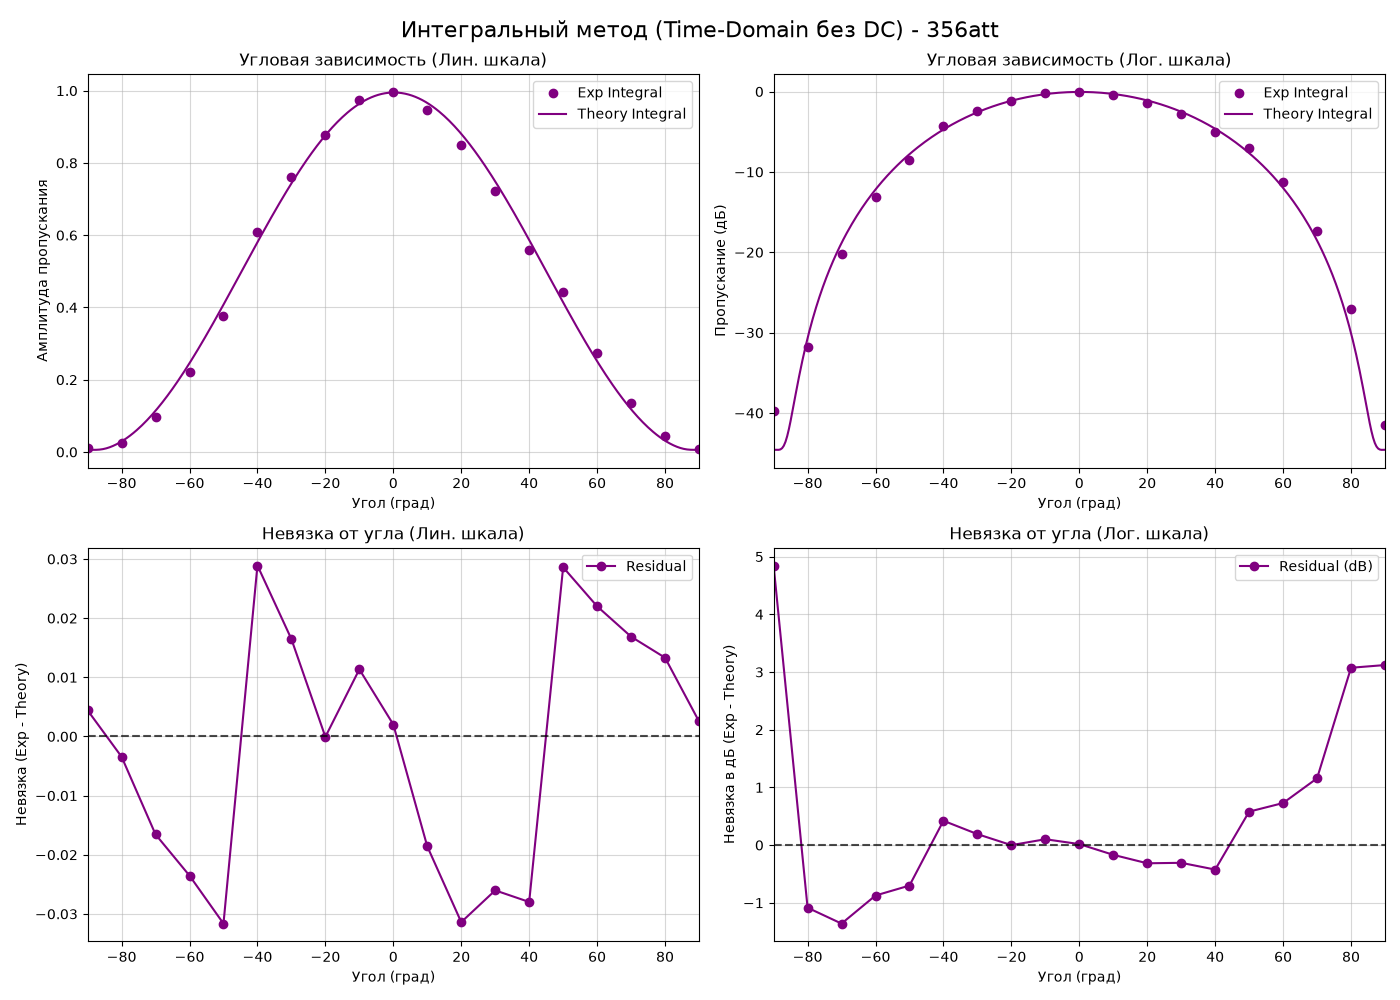
\includegraphics[width=0.48\textwidth]{grid_integral_356att.png}
    \caption{356att: спектральный анализ (слева) и интегральный метод (справа).}
\end{figure}

\subsection{Серия series3}
\begin{figure}[H]
    \centering
    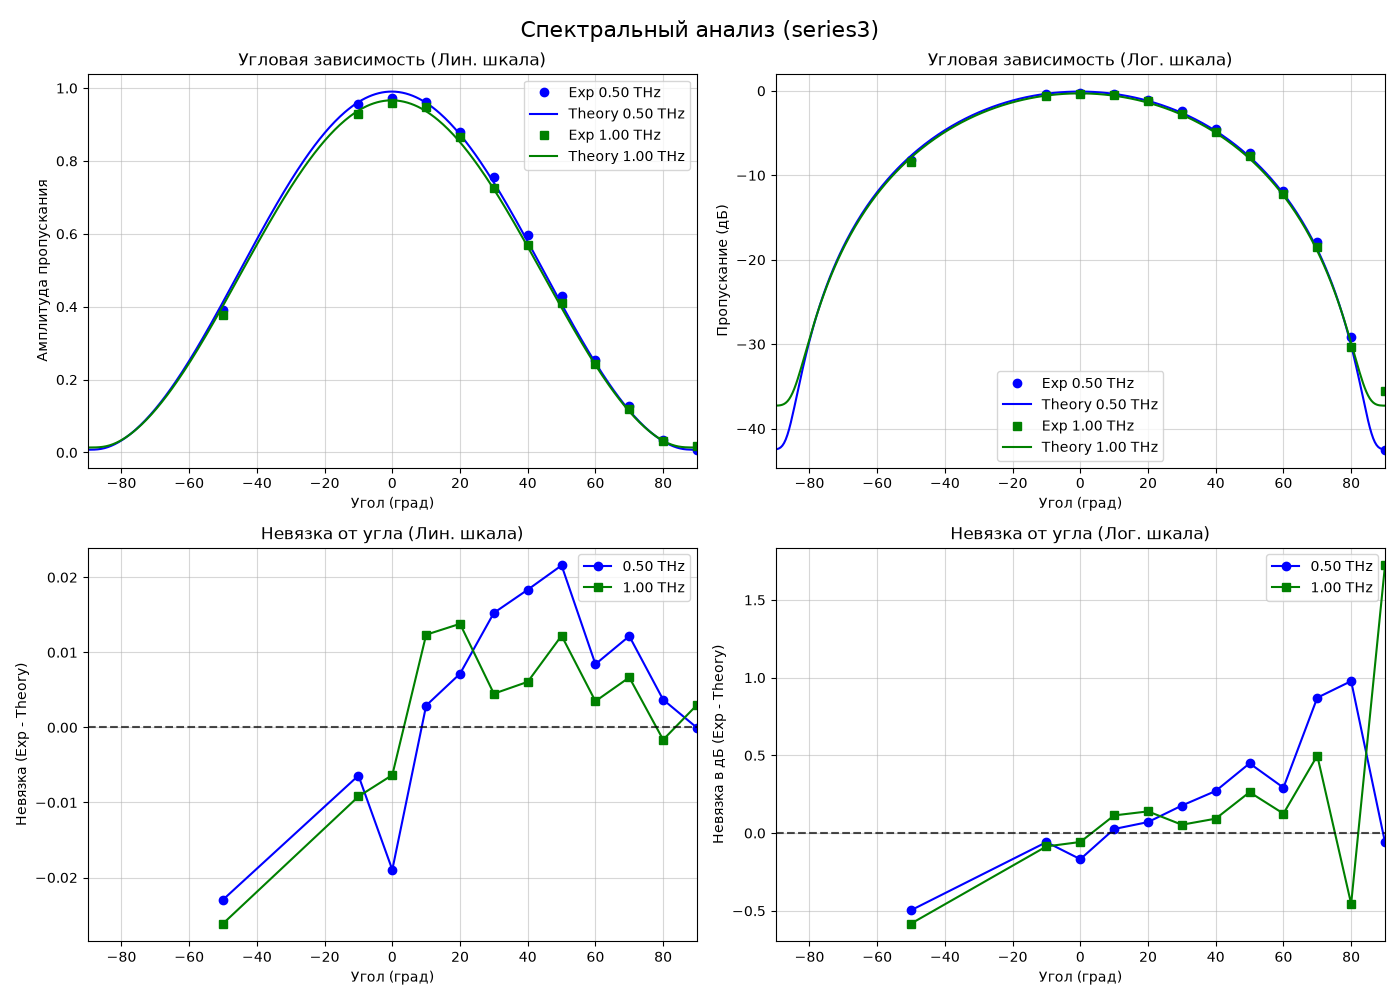
\includegraphics[width=0.48\textwidth]{grid_spectral_series3.png}
    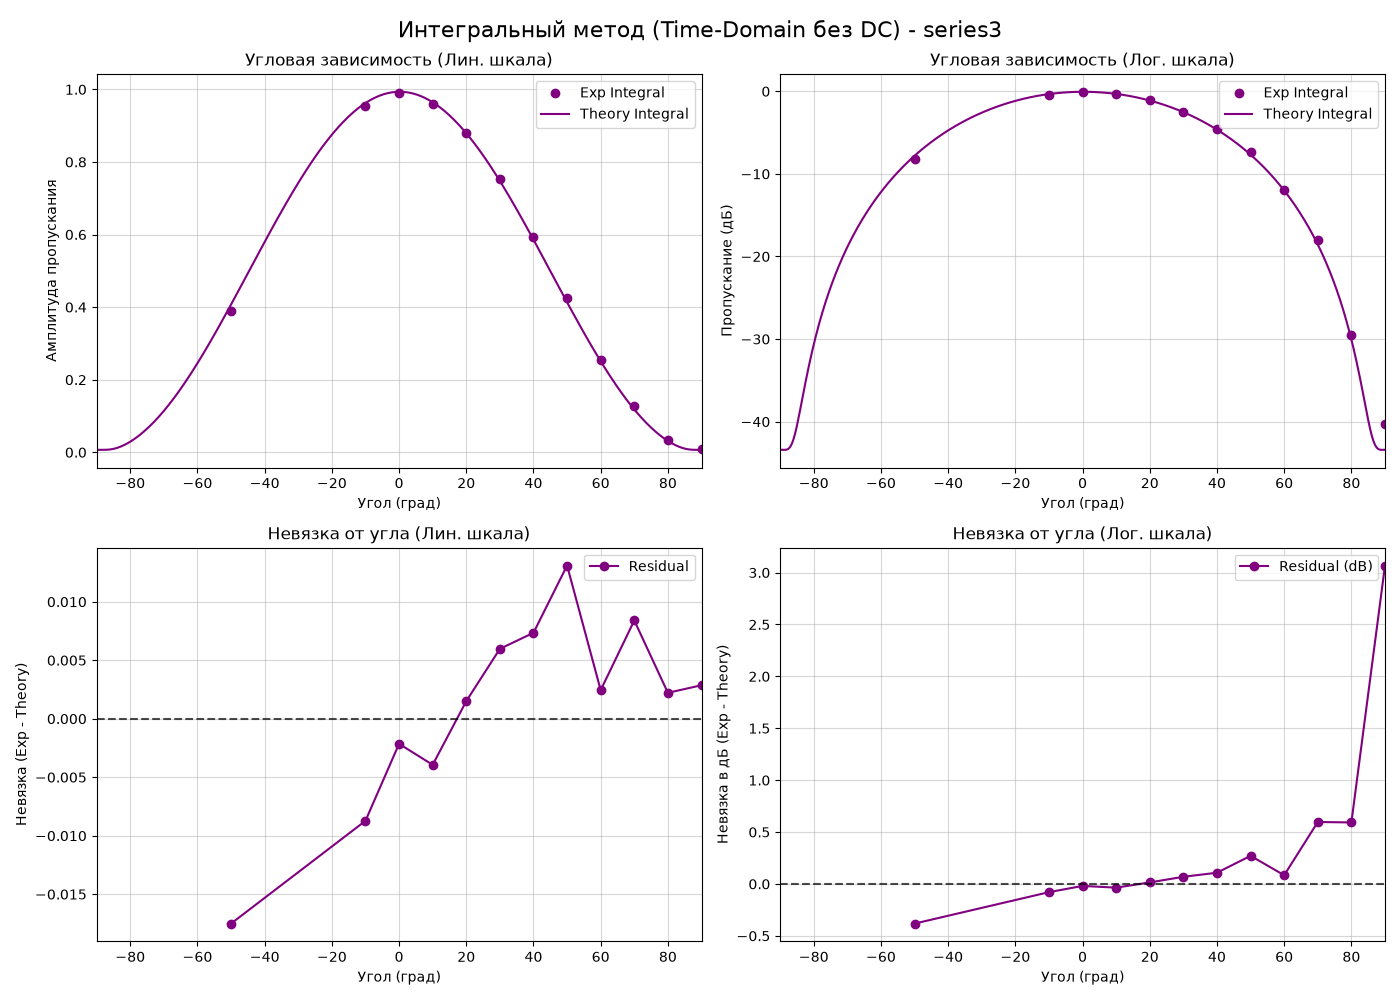
\includegraphics[width=0.48\textwidth]{grid_integral_series3.png}
    \caption{series3: спектральный анализ (слева) и интегральный метод (справа).}
\end{figure}

\section{Комплексный анализ невязок и корреляций}
После пересчета невязок со свободным периодом $P$ глобальная взаимная фазовая корреляция составила $R_\phi = 0.5834$ ($58.3\%$), а амплитудная — $R_A = 0.3029$ ($30.3\%$). 

Сохранение высокого уровня взаимной корреляции фазовых невязок доказывает, что свободный подбор $P$ и $D$ не убирает пространственные погрешности юстировки и краевую дифракцию пучка на оправе, которые носят чисто инструментальный характер.

\section{Заключение}
Свободный подбор шага $P$ в физически обоснованных границах позволил уточнить эффективные параметры решеток. Найденный эффективный шаг ($16.7\text{--}17.5$ мкм) и уменьшенный диаметр нитей ($4.8\text{--}5.0$ мкм) должны использоваться при юстировке и калибровке поляризационных головок в ТГц трактах.

\end{document}
